\chapter{Evaluation\label{chap:evaluation}}


%Explain simulation and communication
%Evaluate different models task based
%How where the realisations/ideas tested?
%What were the results of those tests?

The implementations of the developed concepts were evaluated with regard to the three requirements stated in the introduction: 

\begin{itemize}
\item Update models incrementally during the interaction
\item Predict future object states
\item Incrementally reach a given target configuration
\end{itemize}

In order to evaluate these requirements, the implementations are tested in two different tasks using a physics simulation which is explained in section \ref{sec:environment}. The first task, the \textit{Push Task Simulation}, tests the forward models of the different implementations. The actual task as well as the results achieved in that task are explained in section \ref{sec:pushTaskSim}.
The second task, \textit{Move to Target}, tests the implementations' ability to move an object towards a given configuration. This task and its results are explained in section \ref{sec:moveToTarget}.

\section{Simulation and environment \label{sec:environment}} 

The models are supposed to learn object manipulation through interaction.
The developed prototype implementations are tested in a simplified simulation. For this work gazebo \cite{gazebo} version 2.2.3 was used with the physics engine Open Dynamics Engine (ODE) \cite{ode}.
Gazebo simulates physics one step at a time at fixed time intervals. It is possible to configure the maximum \textit{step size} for each update step as well as the number of steps to be performed in one second in real time (\textit{real time update rate}). 
The simulation time depends on these two values. For this thesis, the standard step size of 0.001 simulation seconds is used. This value represents the timestep which is used to predict the next state of the simulation. 
The real time update rate, which determines how many steps are performed in one real time second, is used to control the speed at which the simulation actually runs. 
This thesis uses an update rate of 500 when the models are to be updated at 100Hz in simulation time. This setting requires the models developed in Python to finish all their updates and queries within 0.02 seconds before the next update.
The simulation sends information about the objects every x simulation steps, where x depends on the chosen update rate and step size. When using 100Hz, the simulation publishes the objects' information every 10 steps of physics simulation.

A very simple two dimensional environment is used, only containing a spherical actuator and a rectangular cube object such as the one that can be seen in figure \ref{fig:gazeboWorld}. In all but one testing scenarios only one of two possible block objects is used mainly due to the reasons discussed in sections \ref{sec:interactionTheory} and \ref{sec:gateTheoDisc}.
The dimensions of all objects as well as their friction coefficients used by the physics simulation are listed in table \ref{tab:environmentObjects}.
The fairly high friction coefficient for the blocks was chosen in order to better suit the assumption of the object state model. By increasing the friction the blocks are less likely to slide. The high mass for the actuator was chosen so that the used velocities actually move the other object since forces are not set directly.

The used action primitives were chosen based on their ease of implementation in the simulation, since it is quite easy to change the global velocity of an object
at runtime. For simplicity the spherical actuator's orientation is fixed to 0 so that the global velocities always correspond to the local coordinate system of the actuator.

\begin{table}
	\centering
	\begin{tabular*}{\textwidth}{@{\extracolsep{\fill} } c c c c c}
			\hline \textbf{Object} & \textbf{Dimension} & \multicolumn{2}{c}{\textbf{Friction coefficients}} & \textbf{Mass} \\ 
			\multicolumn{2}{c}{} & $\mu_1$ & $\mu_2$ & \\
			\hline \hline 
			 Actuator & $0.025m$ & 0.01 & 0.01 & 10\si{\kg} \\
			 Blue rectangular block & $0.5m \times 0.1m \times 0.1m$ & 0.9 & 0.9 & 1\si{\kg} \\  
			 Red square block & $0.3m \times 0.3m \times 0.1m$ & 0.9 & 0.9 & 1\si{\kg} \\  
			\hline 
	\end{tabular*} 
	\caption{Summary of the dimensions, friction coefficients and masses for the objects in the environment. If only one dimension is given, it represents a radius for a spherical object. Three dimensions correspond to the width, depth and height of an object respectively.}
	\label{tab:environmentObjects}
\end{table}

\begin{figure} 
	\centering
	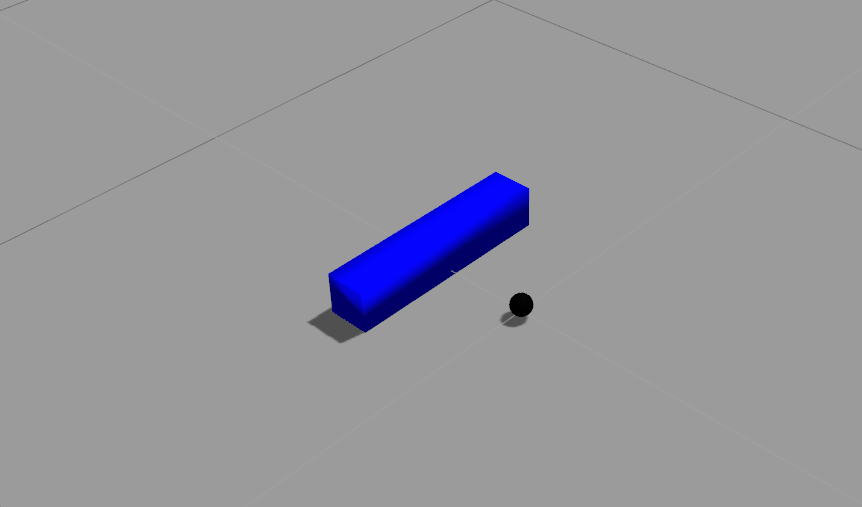
\includegraphics[width=10cm]{gazeboWorld.png} 
	\caption{Overview of the used environment. The black sphere represents the actuator, the models can control using action primitives. The blue square represents the object that the actuator interacts with.}
	\label{fig:gazeboWorld}
\end{figure}


\subsection{Communication}
Gazebo uses a client-server architecture. The actual simulation is being performed by the server.
This server publishes Google Protobuf \cite{protobuf} messages via TCP/IP. Interested clients, for example a graphical user interface, can register themselves as listener to messages of desired types. 
It is also possible to send messages to the server in order to influence the simulation. 

The server can furthermore be extended by writing custom plug-ins that handle self defined messages or perform some sort of additional computation at each update step of the simulation. 

In order for the Python prototypes to communicate with the simulation, an interface on both sides was created.

On the side of the simulation, a custom server plug-in was written. This plug-in publishes the information described in table \ref{tab:availInformation} in the realization chapter at the fixed rate described above. 
The information for all objects is packed into a custom Protobuf message, which is explained in details in Appendix \ref{sec:protobufMessages}. Basically, this message simply contains a list of object descriptions where each object description contains the information explained in table \ref{tab:availInformation}.
Furthermore, the plug-in receives custom control messages. These messages allow the Python interface to influence the simulation.
While the exact messages are explained in the Appendix \ref{sec:protobufMessages}, table \ref{tab:commands} gives an overview about the possible commands, that can be send to the simulation.

On the Python side, an interface was written with the help of the module  pygazebo\footnote{Pygazebo is a Python module developed by Josh Pieper: \url{https://github.com/jpieper/pygazebo} (Last accessed November 2015).}, which provides Python bindings for the message passing system used by gazebo. This interface handles the messages that are received from and send to the simulation. 
At each update step, the interface performs four to five actions:
\begin{enumerate}
\item Construct a suitable worldstate from the provided information
\item Update the model with the current worldstate
\item Get an action primitive from the model given a target configuration
\item Get a prediction about the next worldstate from the model using the current worldstate and chosen action primitive
\item Send the current action primitive to the simulation
\end{enumerate}

The 3rd step is only performed in the tasks evaluating the inverse model. In the \textit{Push Task Simulation} a fixed action primitive is predetermined.

Furthermore, the Python interface provides the testing framework of setting up the models and managing training and testing runs as explained in detail below.

\begin{table}
	\centering
	\begin{tabular}{|c|c|}
		\hline \textbf{Command} & \textbf{Meaning} \\ 
		\hline Move Command & Sets the velocity for the actuator \\ 
		\hline Pause & Pauses the simulation \\
		\hline Continue & Continues the simulation \\
		\hline Reset & Resets all objects to starting configuration \\
		\hline Set Pose & Places a specified object at a certain position and orientation \\
		\hline
	\end{tabular} 
	\caption{Overview of all implemented commands to influence the simulation.}
	\label{tab:commands}
\end{table}

\subsection{Sources of noise \label{sec:noise}}

Although the object's attributes can be read accurately from the simulation, some random noise is still present in the data received by the prototypes: 

1) The physics simulation and the sensors that record the objects' attributes are run in different threads within the simulation. These threads cannot always be perfectly synchronized which can result in minor differences in consecutive timesteps. 

2) The physics simulation itself might encounter numerical instabilities, especially when computing resting forces. These instabilities
might lead to small oscillations within an object's features, such as position. In order to filter out such small noise, all
information from the simulation is rounded to 3 decimal places while constructing the worldstate. 

3) The strongest variation comes from the fact that the implementation communicates with the simulation via asynchronous messages. 
All runs start in a configuration where all objects are resting. In the very first update step, the Python interface sends the first
action primitive to the simulation, which results in the actuator moving. However, the exact time when the simulation retrieves and executes
the action is not deterministic. Depending on the system's load the simulation might have already performed 5 update steps before
it receives and executes the action. In this case, the action affects only half of the update steps. In another situation, the action might
be executed earlier. From the model's point of view, the same action was performed from the same initial situation, but the resulting changes in object states can differ greatly. 

Since this thesis considers a rather simple scenario and these three sources of noise are already present due to the used technologies,
no additional artificial noise was introduced to the system. Both models are expected to be flexible enough to learn from the noisy data without
fixating on outliers.

\section{Push Task Simulation \label{sec:pushTaskSim}}

The \textit{Push Task Simulation} is designed to test the accuracy of the forward model of both concepts. 

\subsection{Scenario description}

In this task, the actuator is controlled by a constant action primitive which first moves the actuator towards an object and then pushes it.
In order to evaluate different interactions, the actuator starts at different starting positions on a line parallel to the object. 

The distance between the starting line and the center of the object is 25 cm. With the used speed, the actuator reaches the object in about 35 update steps after the start of a run. Depending on the third issue explained above, this number can vary a little.

After 150 update steps, a \textit{run} ends and the objects are reset. This means, that the object will be placed at its resting position and the actuator is moved back to the starting line. 

During a run, the object's status can change in a number of ways. In case the actuator goes past the object, it will not change at all. If it is pushed in the center, it will be translated up to \m{0.6}. Furthermore, depending on where the object is pushed, it will be rotated up to \rad{1.02} (around 58°) in either direction. %TODO only true for the blue object
The maximum rotation is experienced when the actuator starts around \m{0.105} away from the origin.

An example starting and end configuration can be seen in figure \ref{fig:pushTaskSim}. 

As the name suggest this task is designed to evaluate the prediction performance of the models during the pushing interaction. The \enquote{simulation} part of the name comes from the fact, that the models will make consecutive predictions based on their last prediction. At the start of each run, the models will make their first prediction based on the current worldstate provided by the simulation. This prediction is then used to construct an appropriate next worldstate which is used at the next update step from the simulation.
Furthermore, the predicted states of both the actuator and the object are send to the simulation for visualization as can be seen in figure \ref{fig:pushTaskSim}.

\begin{figure}
	\centering
	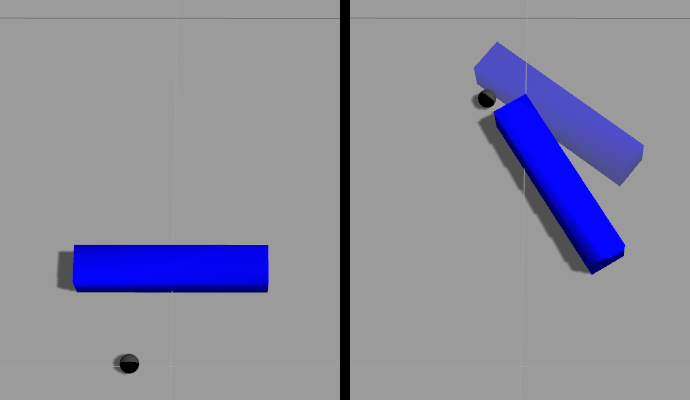
\includegraphics[width=0.8\textwidth]{PushTaskSim.png}
	\caption{Exemplary start and end configuration of a \textit{Push Task Simulation} run. The left side shows the start configuration, while on the right the corresponding end configuration can be seen.
		The opaque objects (dark blue and black) represent the actual block and actuator, while the transparent objects symbolize the predicted states of the objects.}
	\label{fig:pushTaskSim}
\end{figure}

The models will not get any feedback from the real environment in this setting during testing, which means that they will not be able to adapt their predictions based on the actual interaction. The only exception to this is the adapted experiment mentioned below.

In order to be able to make predictions at all, the model will first perform a number of training runs. During these training runs, the models are provided with the current worldstate from the simulation in order to train their local models.

In all runs, an action primitive is used that sets the velocity of the actuator to $0.5\frac{m}{s}$ straight upwards. Although only a constant global action is used, the prediction task is still challenging enough: \\
The constant action primitive does make it easy for the object state concept to learn the forward model of the actuator. However, the local forward model for the object is not as simple because the velocity is not constant in local coordinates but rather depends on the object's orientation. 
Similarly, in the interaction concept the used action primitive is also transformed to the local coordinate frame of the reference object.

Different kinds of training scenarios are evaluated in this task which are further explained below when their results are presented.


\subsection{Evaluation criteria}

This task tries to evaluate the precision of the different models. In order to measure this precision, the distance between the predicted and the actual object state is computed at the end of each test run.
In this scenario, the models predict up to two quantities: The position and the orientation. 

Finding a metric that can adequately combine differences in position and orientation at the same time is difficult. Furthermore, the interpretation of such a measurement is not intuitive. Therefore, the differences in position and orientation are considered separately. 
The positional difference is computed by the euclidean distance between the centers of the predicted and the actual object. The difference in orientation is given by the absolute difference between the predicted and the actual orientation.

Each training and testing setting is repeated 20 times and the average differences in position and orientation as well as their standard deviations are reported. 

\subsection{Evaluated configuration}
%TODO
The implementations of both concepts offer several possible configurations, ranging from using different features to using hard coded components in the gating concept and choosing different learning rates for the underlying regression and classification models. 

Since the goal of this thesis was to provide models that adapt to their environment with as little prior knowledge as possible, standard parameters are where possible. This includes setting all learning rates to zero for the \gls{aitm}. This choice is corresponds to disabling the adaptation within the \gls{aitm}.
Some meta parameters, such as $\eta_{max}$ had to be predetermined and adapted to the given situation beforehand.

In order for both models to be more comparable, the local actuator models as well as the gating function were also learned online in the object state concept, even though it is possible to provide accurate models by hand in this situation.

In this evaluation, the implementations are evaluated in the configuration described in the last chapter with meta parameters chosen as indicated by table \ref{tab:parameters}.
Both models use almost the same set of meta parameters. While the interaction model specifies $\epsilon_{noise}$ to determine the set of changed features, the object state model uses $\epsilon_{change}$ to determine when an object state has changed.

\begin{table}[H]
	\centering
	\footnotesize
	\begin{tabular*}{\textwidth}{@{\extracolsep{\fill}} c c c }
			\hline 
			& \textbf{Parameter} & \textbf{Value}  \\ 
			\hline \hline 
	 		 Simulation & Step size & 0.001 s  \\
			 & Real time update rate & 500 \\
			 & Update rate models & 100 Hz \\
			 & Number decimals & 3  \\
			 \hline
			 \gls{aitm}& $\sigma$ & 0.05 \\
			 & $\epsilon_{max}$ & 0.001\\  
			 & $\eta_{in}$ & 0 \\
			 & $\eta_{out}$ & 0  \\
			 & $\eta_{A}$ & 0  \\
			 \hline
 			 Episodes & $\epsilon_{noise}$ & 0.01  \\
 			 \hline
 			 Gating function & $\epsilon_{change}$  & 0 \\
 			 \hline
 			 \gls{tiim} & $\epsilon_{index}$ & 0.002  \\
 			 & $\epsilon_{Node}$ & 0.001  \\
 			 & Number of differing dimensions  & 1  \\
 			 \hline
			 Move To Target & $\epsilon_{close}$ & 0.1  \\
			 & $\epsilon_{closeEnough}$ & 0.01 \\
			\hline 
	\end{tabular*} 
	\caption{Summary of the meta parameters used for the presented evaluations. The learning rates $\eta_x$ are the same for all instances of the \gls{aitm}.}
	\label{tab:parameters}
\end{table}

\subsection{Results}

\textbf{Generalization on random training data:}

%TODO if another object is added, specify which one is used here
The first test evaluates the prediction accuracy against the number of random training runs. The training run start positions were chosen at random in the range of \m{-0.25} to \m{0.25}. This means that they span the entire width of the block objects.
For each number of training runs that were evaluated, 21 test runs were performed with starting positions in the range of \m{-0.35} to \m{0.35} at \m{0.035} intervals. This means that 6 test runs went past the object without interacting with it.
The averaged results for the blue block predictions over all folds for the interaction state model in the first configuration can be seen in figure \ref{fig:learnCurveInteraction1}. The averages over all test positions as well as only over the 15 central test positions are shown.

\begin{figure}[h]
\centering
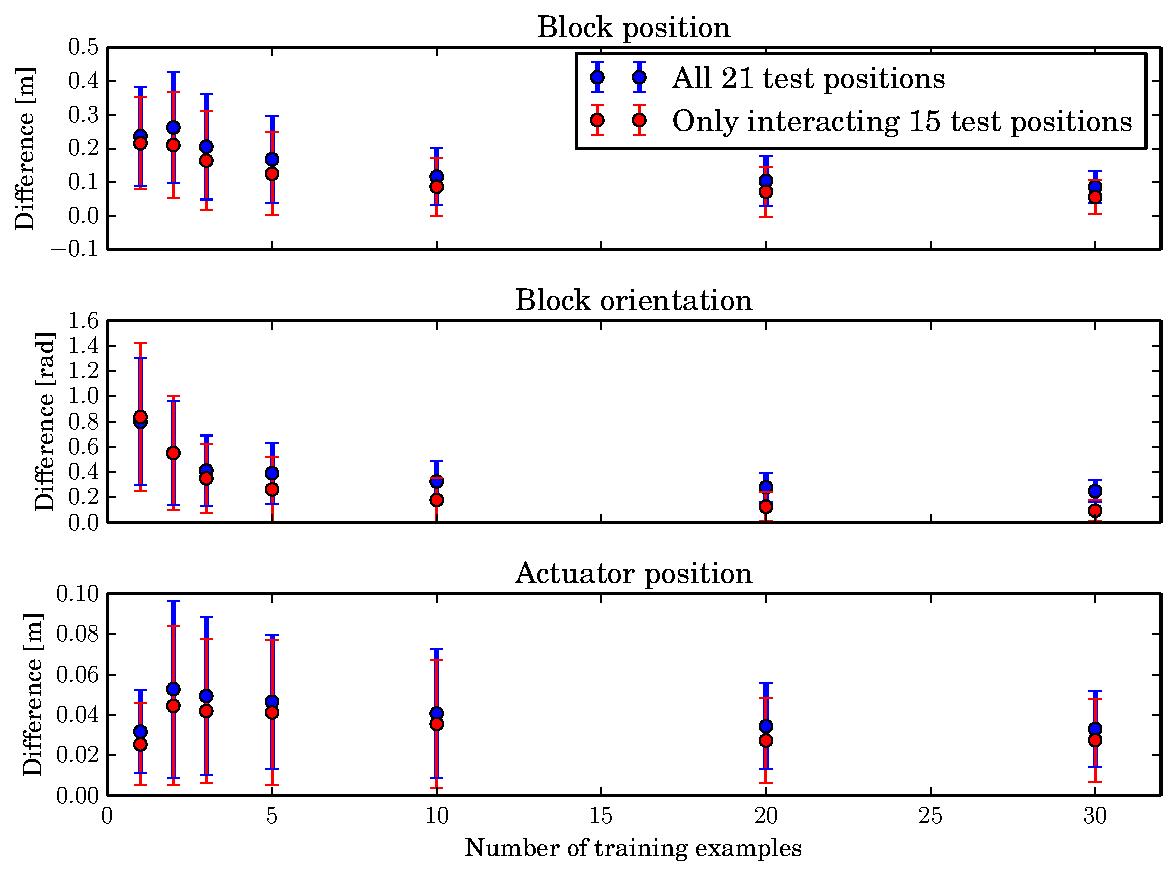
\includegraphics[width=0.7\textwidth]{LearningCurveinteractionModel_C_0E20FoldsSigma005.pdf}
\caption{Learning curve for the interaction concept with the blue block. Difference in position and orientation for the block predictions and differences for the actuator position at the end of a run are shown. Error bars indicate one standard deviation. Blue error bars represents averages over all 21 test positions, while red error bars only averages over the 15 test positions where the block is actually moved.}
\label{fig:learnCurveInteraction1}
\end{figure}

The positional prediction error starts around \m{0.24} with a standard deviation of around \m{0.15} when the model is only trained with a single training example. The prediction performance improves to roughly \m{0.09} with a standard deviation of around \m{0.05}.
The predicted orientation error starts at an average of about \rad{0.8} with a standard deviation of \rad{0.5} but improves to around \rad{0.25} with a standard deviation of \rad{0.09} when increasing the number of random training examples.
The performances for position and orientation do not increase much more after the first 10 training runs (\m{0.12} $+/-$ \m{0.08} for position and \rad{0.33} $+/-$ \rad{0.16} for orientation).
The actuator position predictions errors are ranging between \m{0.03} and \m{0.05} with standard deviations between \m{0.02} and \m{0.04}.

When only considering the testing positions where the actuator actually interacts with the block (red error bars), predicted errors improve slightly.

The results for the same experiment with the object state with gating function model using the first configuration are presented in figure \ref{fig:learnCurveGate1}.

\begin{figure}[h]
\centering
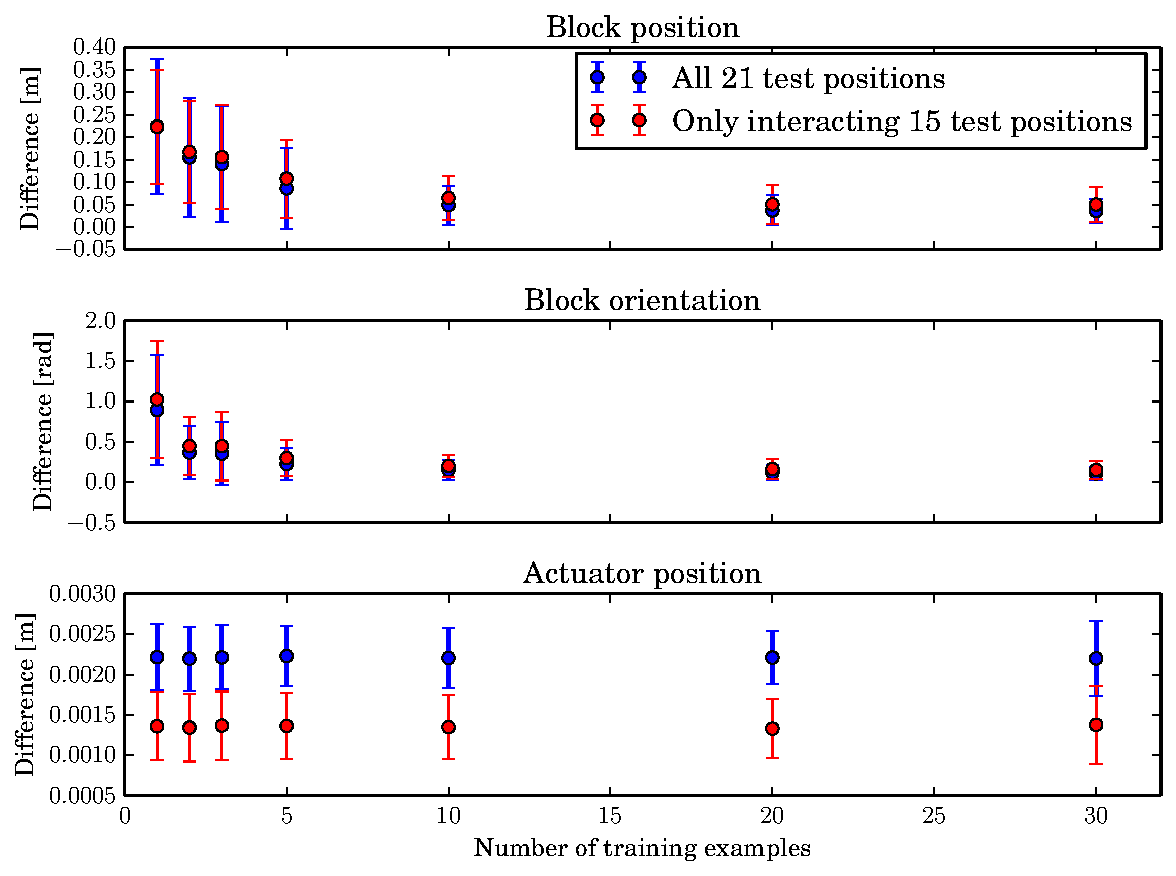
\includegraphics[width=0.7\textwidth]{LearningCurvegateModel_C_0E20FoldsAllGateFSigma005.pdf}
\caption{Learning curve for the object state with gating function concept using the blue block. Difference in position and orientation for the block predictions and differences for the actuator position at the end of a run are shown. Error bars indicate one standard deviation. Blue error bars represents averages over all 21 test positions, while red error bars only averages over the 15 test positions where the block is actually moved.}
\label{fig:learnCurveGate1}
\end{figure}

The positional prediction error over all testing positions (blue error bars) starts at around \m{0.22} with a standard deviation of \m{0.15} for only one training run in the object state with gating function model. By increasing the number of random training runs to 30, the positional error reduces continuously to around \m{0.04} with a standard deviation of only around \m{0.03}.
The predicted orientation error starts at around \rad{0.89} with a standard deviation of \rad{0.68}.
After 30 test runs an error of \rad{0.10} with a standard deviation of \rad{0.08} remains.
For this model the performance increases only slightly after having seen 10 training runs for both the error in position (\m{0.05} $+/-$ \m{0.04}) as well as orientation (\rad{0.18} $+/-$ \rad{0.12}).
Predictions for the actuator position are fairly constant around \m{0.002} with a standard deviation of around \m{0.0004}.

Unlike in the other model, prediction errors are slightly worse for the block position and orientation when only considering the 15 testing positions where an actual interaction takes place. However, actuator prediction are slightly more accurate (average error improves by about \m{0.001}).

Memory-based regression methods such as \gls{nn} approaches often suffer from the increasing computational complexity as the number of training samples increases.
Table \ref{tab:learnCurveInteractionNodes} presents the average numbers of update calls and the number of nodes in the \glspl{aitm} used by the interaction state model after training. Since the number of learned \glspl{ac} varies between the runs, only the number of nodes for the \gls{ac} with the most nodes is recorded. Only 149 update calls are made at most for each run because the models are not updated after the 150th timestep.

\begin{table}
\footnotesize 
	\centering
	\begin{tabular*}{\textwidth}{@{\extracolsep{\fill}} c c c c c c}
			\hline \textbf{Train runs} & \textbf{AC Updates}&  \textbf{AC Nodes} & \textbf{\# ACs} & \textbf{ACS Updates} &\textbf{ACS Nodes} \\ 
			\hline \hline 
			 1 & 59.74 (7.93) & 17.58 (13.14) & 6.9 (0.45) & 149 & 39.65 (11.49) \\
			 2 & 98.37 (24.63) & 28.32 (21.68) & 9.58 (1.93) & 298 & 85.45 (17.22) \\  
			 3 & 132 (27.26) & 28.9 (19.10) & 10.37 (2.25) & 447 & 124.35 (22.57) \\
			 5 & 224.84 (29.69) & 51.05 (25.84) & 11.42 (2.23) & 745 & 196.75 (29.23) \\
			 10 & 453.37 (62.96) & 106.21 (61.37) & 12.63 (2.98) & 1490 & 372.55 (21.93) \\
			 20 & 876.11 (78.19) & 182.53 (94.63) & 15.58 (1.09) & 2980 & 740.15 (47.08) \\
			 30 & 1209.89 (146.47) & 239.42 (130.38) & 16.32 (1.03) & 4470 & 1086.95(76.74) \\
			\hline 
	\end{tabular*} 
	\caption{Record of the average number of nodes that resulted from the recorded number of update calls in the regression and classification \gls{aitm} for the interaction model. Only the number of the \gls{ac} with the most nodes is used in each repetition is used to compute the averages for the AC Updates and AC Nodes. Numbers in brackets represent one standard deviation.}
	\label{tab:learnCurveInteractionNodes}
\end{table}

The data in the table indicates, that on \gls{ac} dominates the space since the number AC Updates for the \gls{ac} with the most nodes is significantly bigger than the average number of Update calls divided by the average number of \glspl{ac}.

Similarly, table \ref{tab:learnCurveGateNodes} shows the respective number of update calls and nodes for the \glspl{aitm} used by the object state model.
The \glspl{ac} appear to keep a node for every 3 to 4 update calls. The \gls{acs}, which is trained on every update, also creates a node for about every 4th update.

\begin{table}
\footnotesize 
	\centering
	\begin{tabular*}{\textwidth}{@{\extracolsep{\fill}} c c c c c}
			\hline \textbf{Train runs} & \textbf{Object Updates}&  \textbf{Object Nodes} & \textbf{Gate Updates} &\textbf{Gate Nodes} \\ 
			\hline \hline 
			 1 & 93.5 (16.87) & 26.55 (11.01) & 149 & 3.7 (0.46) \\
			 2 & 194.35 (27.43) & 39.4 (15.87) & 298 & 5.55 (1.07) \\  
			 3 & 287.25 (33.85) & 67.4 (20.44) & 447 & 6.4 (1.07) \\
			 5 & 479.6 (42.91) & 111.95 (20.46) & 745 & 6.8 (1.07) \\
			 10 & 963.7 (37.04) & 219.65 (38.24) & 1490 & 7.75 (0.89) \\
			 20 & 1894.25 (46.3) & 438.2 (45.17) & 2980 & 10.4 (6.88) \\
			 30 & 2883.8 (111.4) & 603.05 (36.16) & 4470 & 10.2 (4.23) \\
			\hline 
	\end{tabular*} 
	\caption{Record of the average number of nodes that resulted from the recorded number of update calls in the regression and classification \gls{aitm} for the object state model. Values in brackets represent one standard deviation.}
	\label{tab:learnCurveGateNodes}
\end{table}

Interestingly, the number of nodes required for the gating function is rather constant whereas the local forward model in the predictor creates a node between every 4th and 5th update call on average. 

The number of nodes learned in the local forward model of the actuator is not included in the table since it only contains two nodes in all runs regardless of the number of training runs. 

\textbf{Generalization on selected training data:}

In order to analyze the information required for generalization, another training scheme was used. This time the models were only provided with three predetermined training runs. The starting positions \m{-0.18}, \m{0.0} and \m{0.18} were used in this experiment. These three were chosen in order to provide the models with examples of both possible rotations as well as the lateral movement. The same 21 test runs were performed as before. This time prediction errors at the end of the run are recorded for each starting position separately. Due to the noise explained above, some randomness is still present in the data which is why this experiment was also repeated 20 times and the average errors are reported. 

The results for the interaction model are shown in figure \ref{fig:eachPosInteraction}.

\begin{figure}
\centering
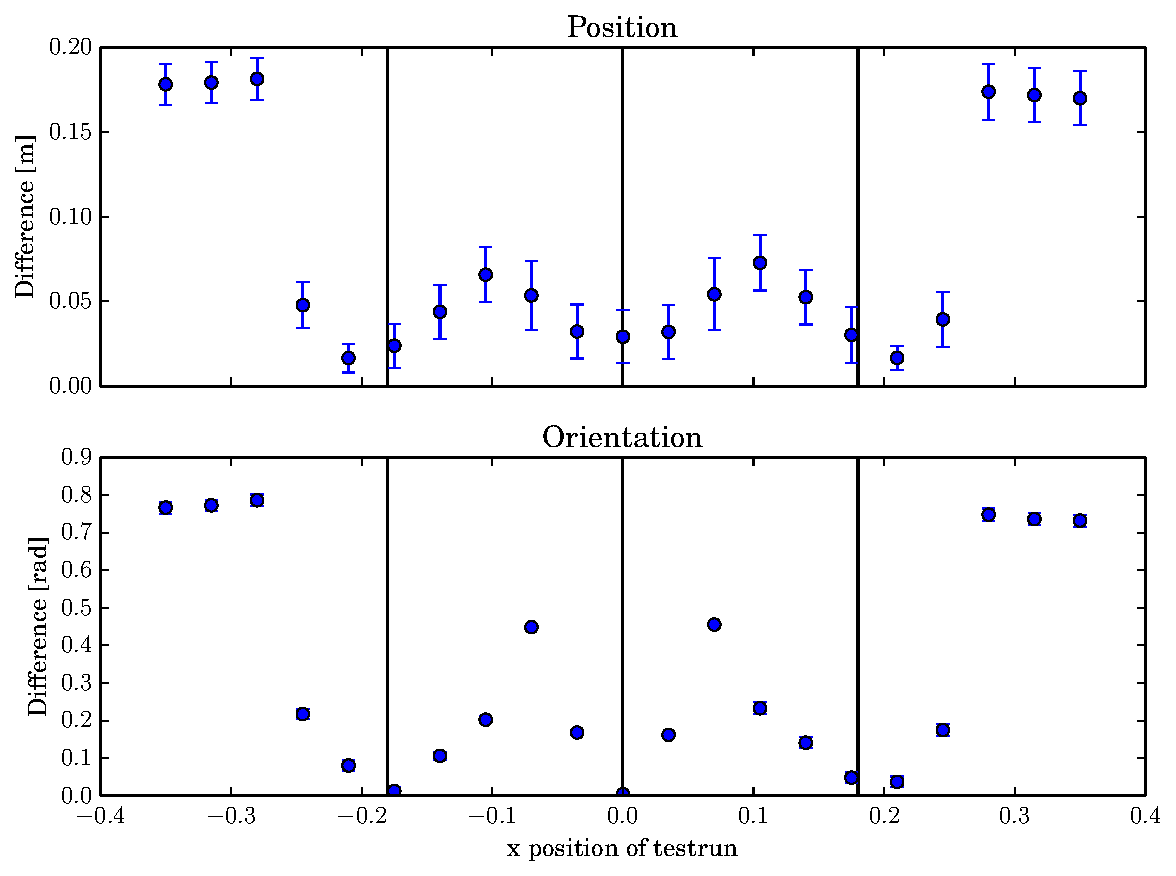
\includegraphics[width=0.7\textwidth]{EachPositioninteractionModel_C_8E20FoldsAllACSFSigma005.pdf}
\caption{Prediction errors for the interaction model at each of the 21 test positions after seeing three exemplary training examples. The training positions are highlighted by the block lines. Error bars indicate one standard deviation.}
\label{fig:eachPosInteraction}
\end{figure}

The predictions for the test runs that do not actually interact with the block, are rather poor. The model predicts an incorrect change in position around \m{0.18} +/- \m{0.01} and in orientation around \rad{0.77} +/- \rad{0.02} on both sides of the object. 
Predictions are quite good close to the seen training examples when the block is actually influenced: The positional error is as low as \m{0.02} +/- \m{0.01} around the two outer training positions and slightly higher for the central position (\m{0.03} +/- \m{0.02}). Generally the same applies for orientation, but the model does not make a prediction error at the central position. At the outer positions slight prediction errors are made (\rad{0.01} +/- \rad{0.01}).
The further away from the training positions, the worse the prediction for both position and orientation becomes. Interestingly, the worst positional prediction of \m{0.07} +/- \m{0.02}  happens \m{0.105} away from the center, while the worst prediction for orientation of \rad{0.45} +/- \rad{0.01} is seen \m{0.07} away from the center.

It is also interesting to note, that the position and orientation are predicted very consistently (most standard deviations below \m{0.02} and all below \rad{0.02}).

The results for the same experiment performed with the object state model are presented in figure \ref{fig:eachPosGate}.

\begin{figure}
\centering
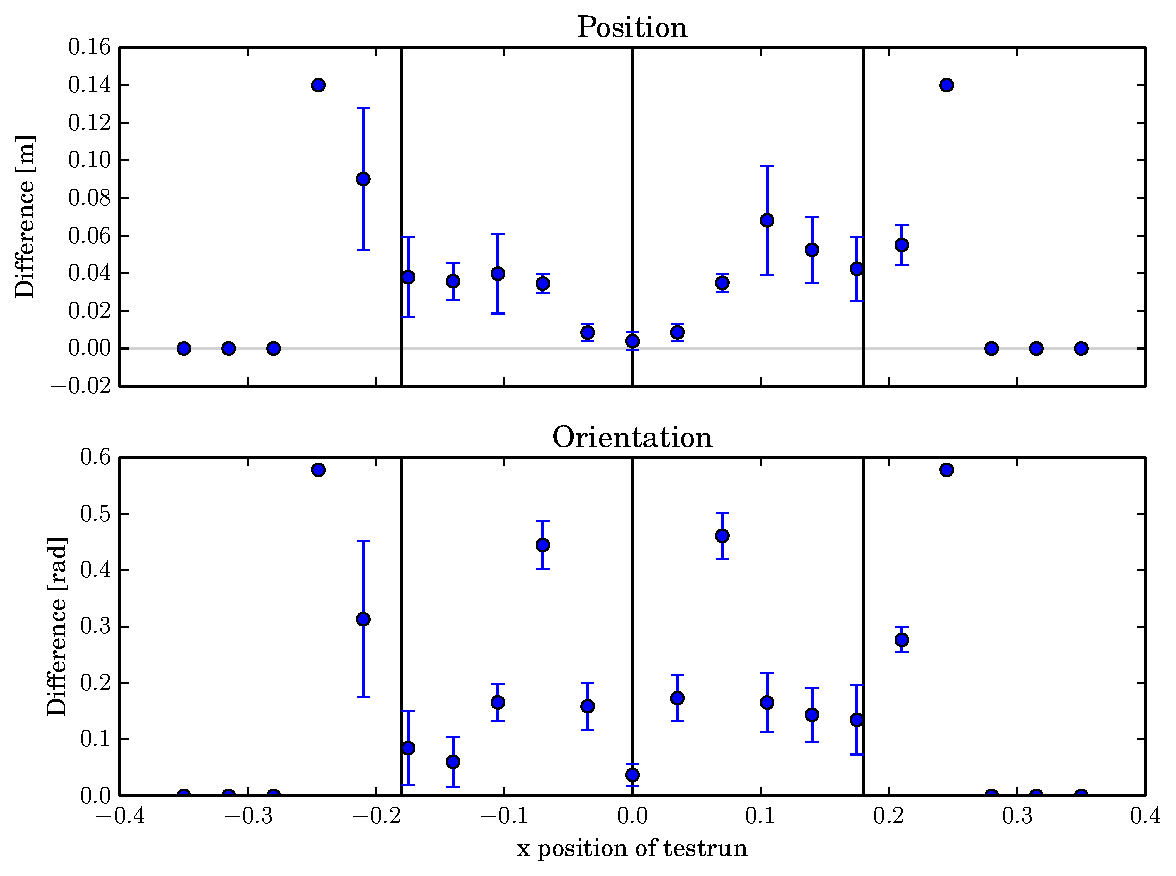
\includegraphics[width=0.7\textwidth]{EachPositiongateModel_C_8E20FoldsAllGateFSigma005.pdf}
\caption{Prediction errors for the object state model at each of the 21 test positions after seeing three exemplary training examples. The training positions are highlighted by the block lines. Error bars indicate one standard deviation.}
\label{fig:eachPosGate}
\end{figure}

The object state with gating function successfully does not make predictions for the test runs that go past the object after seeing the three fixed training runs. However, no predictions are also made for the first interacting test positions on either side which results in constant errors in position of \m{0.14} and in orientation of \rad{0.58}.
For the other test positions that actually interact with the block, the predictions are better for positions close to the training examples as in the other model.
The predicted errors are not quite as symmetric as in the other model.
The central position has a prediction error of close to 0 with a standard deviation below \m{0.01}. 
The predictions for position are slightly more accurate between the left and the middle training position (ranging from \m{0.01} +/- \m{0.0} to \m{0.04} +/- \m{0.02}) when compared to the testing positions between the middle and the right training position (ranging from \m{0.01} +/- \m{0.0} to \m{0.07} +/- \m{0.03}). Outside the training positions, the predictions are better for the 17th testing position than for the fifth one (\m{0.09} +/- \m{0.04} at the fifth and \m{0.06} +/- \m{0.01} at the 17th testing position).

Prediction errors for orientation show a similar trend: 
In the central position the prediction error in orientation is \rad{0.04} +/- \rad{0.02}.
The same outliers for orientation are found as in the other model. The testing positions \m{0.07} away from the center have errors around \rad{0.45} +/- \rad{0.04}.
The remaining errors for orientation in between the training positions are ranging from \rad{0.06} +/- \rad{0.04} to \rad{0.16} +/- \rad{0.05}.
As with the positional prediction, the prediction for orientation is slightly worse for the fifth testing position compared to the 17th one, although both have the same distance to the closest training position (\rad{0.31} +/- \rad{0.14} at the fifth and \rad{0.28} +/- \rad{0.02} at the 17th testing position).

In order to be able to interpret these results, figure \ref{fig:EachPosEndPos} shows final configurations (predicted and actual) for every 2nd testing positions for both models.

\begin{figure}
\centering
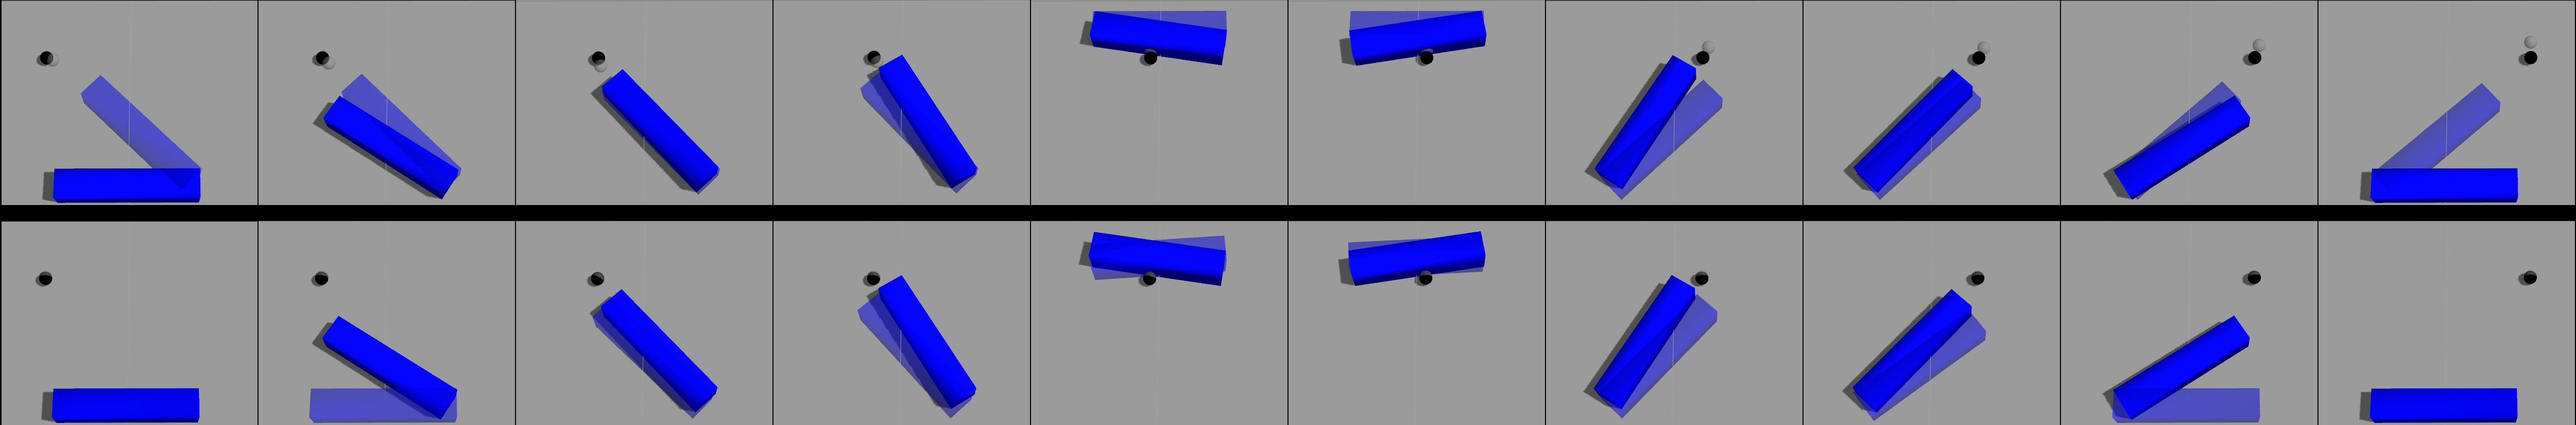
\includegraphics[width=\textwidth]{EachPosEndPos.png}
\caption{Predicted and actual end positions. Transparent objects represent the predictions. Top row shows results for the interaction model, while bottom row shows the results for the object state with gating function model. Every 2nd of the 21 testing positions is shown. The training positions are right next to the third image on either side as well as between the two central images.}
\label{fig:EachPosEndPos}
\end{figure}

The number of required nodes for this experiment is slightly lower then when learning on random data and show hardly any variance. The interaction model consistently trains eight \glspl{ac} of which the biggest one contains around 6 nodes. The \gls{acs} requires 3.5 nodes on average. 
The object state model constantly requires 9 nodes in the gating function and around 58 nodes for the local forward model of the block.

\textbf{Generalization with constant feedback:}

While the previous scenarios test the accumulated prediction error, it is often not required to make accurate predictions 150 steps into the future. Instead it is more important to adapt to changes in the environment quickly. For that reason, a variation of the \textit{Push Task Simulation} was also evaluated. In this variation, the models are not trained before testing, but will instead continuously receive updates from the environment. That way the models online learning capabilities are evaluated. The models will still make consecutive predictions based on their last prediction. Their last predictions are not corrected based on the actual environment and the models do not get or compute any feedback as to how good their last prediction was. 

A qualitative evaluation is provided in figure \ref{fig:pushTaskSim2}. Each row in the figure represents one run as described before. The leftmost images show the initial configuration at the start of the run. The rightmost images show the interaction step where the block prediction changed for the last time. 
The first row shows the first run as performed the object state model. An image sequence for the interaction state model looks almost identical and was therefore omitted. The second row shows the second run performed by the object state model, while the third row shows the same run performed by the interaction state model.

The transparent object represent the last predictions, while the opaque objects represent the actual states of the objects. 
In order to be able to actually see meaningful differences between consecutive interactions, these images where taken in a setting where the model is only updated every 10Hz, meaning that the model was updated and queried every 0.1 seconds in simulation time instead of the 0.01 seconds used for all the other evaluations. No other adaptation to the models was made. 

\begin{figure}
\centering
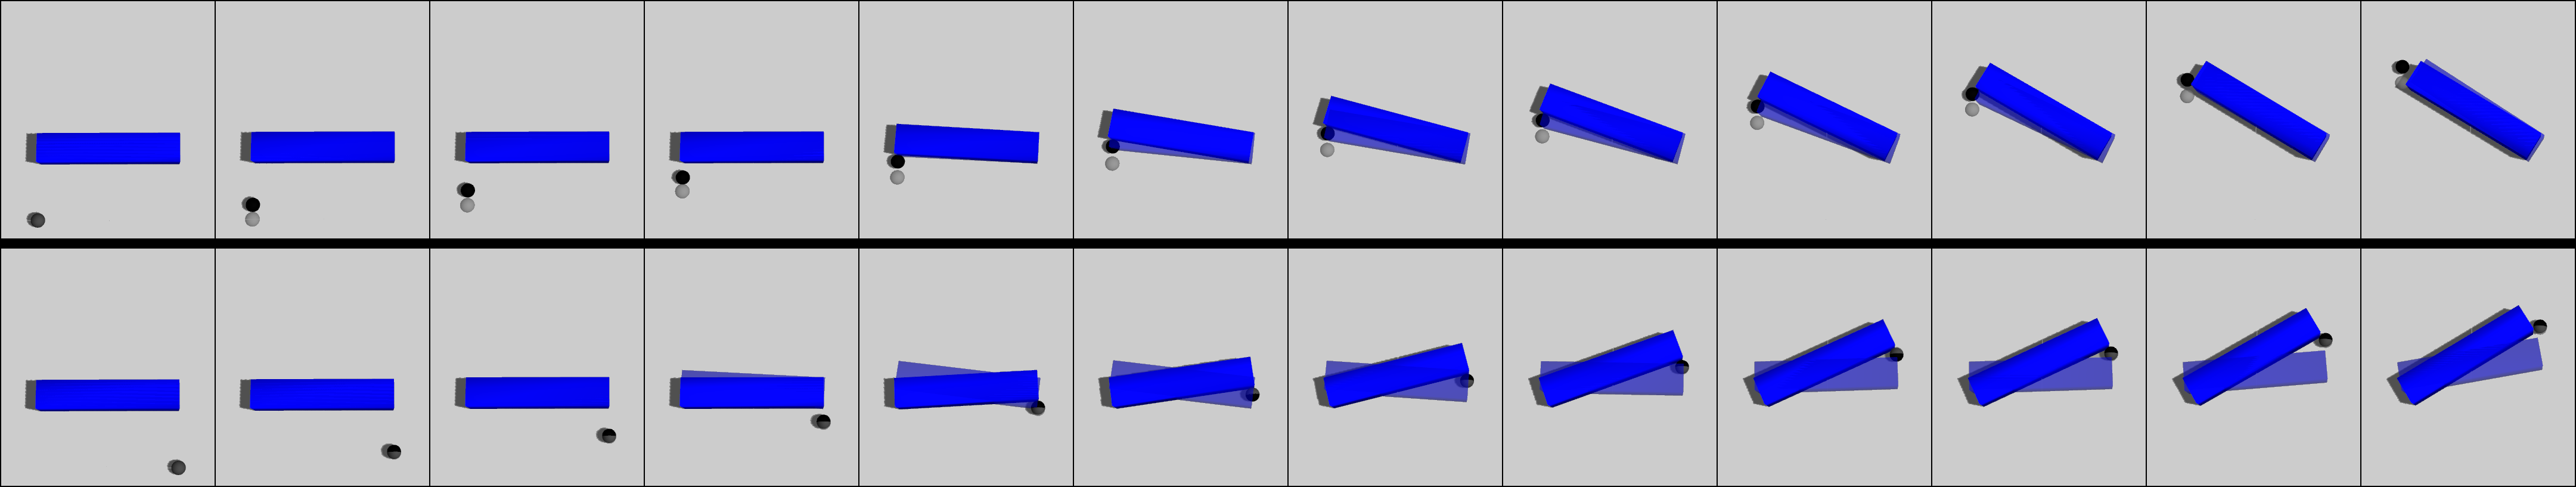
\includegraphics[width=\textwidth]{pushTaskSim2.png}
\caption{Consecutive interactions in the \textit{Push Task Simulation} variation. Top row shows images of the first test run, while the second row shows images of the second test run on the other side of the object. }
\label{fig:pushTaskSim2}
\end{figure}

While no prediction is made for the actuator in the 2nd image of the top row, the actuator is predicted correctly in the 2nd run. The top row continues to lag one frame behind with its predictions. The final block predictions are accurate again.
In the 2nd run, the actuator predictions are good. However, the model predicts the same rotation as in the first run once the actuator comes close to the object. After a few other frames, the predictions start turning in the other direction, but do not catch up to the actual object. The object state model does not change its prediction for the block anymore after the actual actuator passed the actual block. However, the interaction state model continues to make predictions until it reaches the point shown in the image which leads to a better prediction at the end of the run.

\subsection{Extension to multiple objects \label{sec:multipleObjects}}

Environments rarely only contain a single object, however, so far in this thesis, only one object was considered. While it is difficult for the interaction model to handle multiple objects due to the reasons explained in section \ref{sec:interactionTheory}, the object state model handles objects separately anyways. In this evaluation the red block described in table \ref{tab:environmentObjects} is added to the scene and six fixed training positions (three interacting with each object) are used. The blue block remains at the same position as in the previous experiments, while the red block is located left of it with a center position of \m{-0.6} in x direction and \m{0.35} in y direction. This position ensures that the distance from the starting line remains the same compared to the blue object.
The object is then tested on a fixed set of 21 testing positions ranging from \m{-0.8} to \m{0.4} in intervals of \m{0.06}.


The model was not altered in any way for the results presented in figure \ref{fig:eachPosTwoObjects}.

The gating function often classifies incorrectly for the red object, but the blue object does not seem to be influenced by the new object at all since the results are basically identical to the ones presented in \ref{fig:eachPosGate}. 
Within the training positions for the red object, the predictions are fairly good (below \m{0.05} +/- \m{0.02} for position and below \rad{0.09} +/- \rad{0.06}).

By introducing a seventh training position in between both objects, the prediction quality of runs that do not interact with the red object improves due to better performance of the gating function as can be seen in figure \ref{fig:eachPosTwoObjects7Trains}. The other predictions remain mostly unchanged through the introduction of the additional training run.


As in the experiment before, figure \ref{fig:eachPosTwoObjectsEndPos} shows the predicted and actual configuration for every second testing positions in order to allow for easier interpretation of these results.

\begin{figure}[h]
\centering
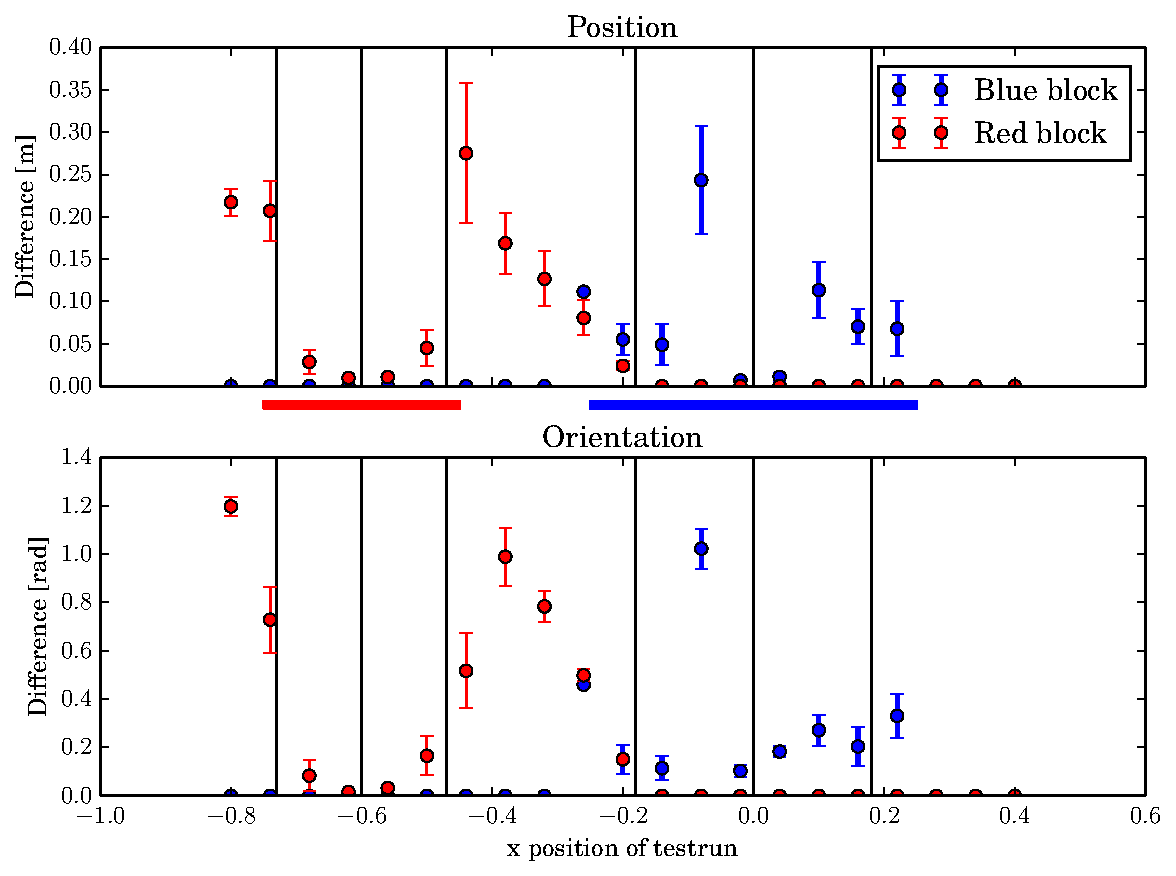
\includegraphics[width=0.65\textwidth]{EachPosgateModel_C_8E20Folds2Objects.pdf}
\caption{Prediction errors for the object state model with two objects. The training positions are highlighted by the black lines. Error bars indicate one standard deviation. The red and blue bar in between the blocks visualize the size and position of the red and blue blocks respectively.}
\label{fig:eachPosTwoObjects}
\end{figure}

\begin{figure}[H]
\centering
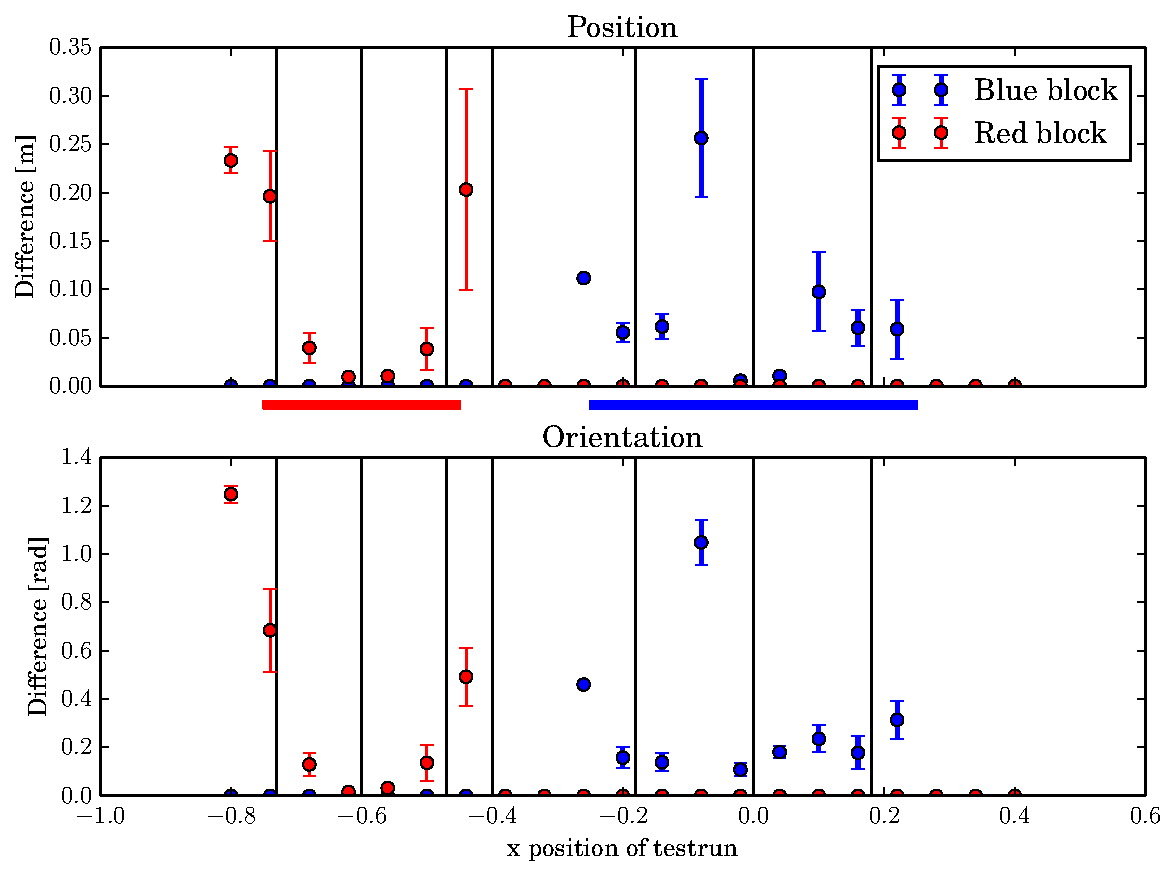
\includegraphics[width=0.65\textwidth]{EachPosgateModel_C_8E20Folds2Objects7TrainV2.pdf}
\caption{Prediction errors for the object state model with two objects with an additional separating training positions. The training positions are highlighted by the black lines. Error bars indicate one standard deviation. The red and blue bar in between the blocks visualize the size and position of the red and blue blocks respectively.}
\label{fig:eachPosTwoObjects7Trains}
\end{figure}

\begin{figure}[h]
\centering
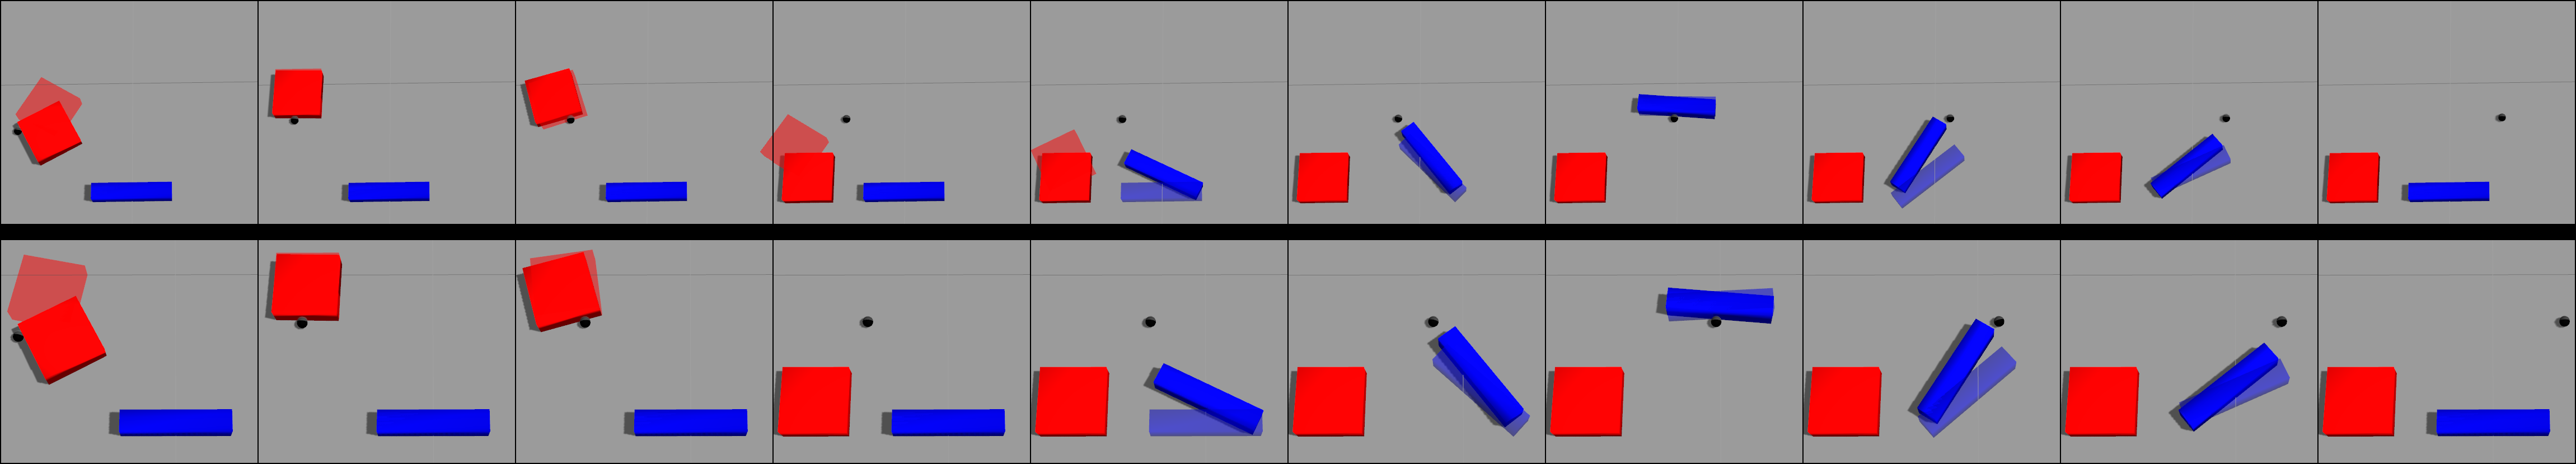
\includegraphics[width=\textwidth]{EachPos2ObjectsEndPos.png}
\caption{Predicted and actual end positions for the two object scenario. Transparent objects represent the predictions. The top row shows the results after having seen six training runs. The bottom row shows the results for the experiment adding a seventh training run in between both objects. Every 2nd of the 21 testing positions is shown.}
\label{fig:eachPosTwoObjectsEndPos}
\end{figure}


\section{Move to Target \label{sec:moveToTarget}}

The \textit{Move to Target} task is designed to evaluate the concept's ability to reach a given target configuration incrementally. AS mentioned in the 
realization chapters of both models, this thesis assumes that the inverse model has been sufficiently trained, i.e. it has seen all required changes in feature dimensions, before a target is specified. 

\subsection{Scenario description}

In this task only a target configuration for the blue block object is given to the models. At each update step the models are updated with the current worldstate.
This means that they can adapt their inverse model during testing.
Afterwards, the interface queries the model for the next action primitive which is then send to the simulation. This is repeated until the target configuration is reached or a maximum number of steps of 3000 has been performed.
The models consider a target configuration as reached, if the norm of the difference vector between the target representation and the current situation is smaller than 0.01. This means, that the combined vector of positional difference as well as difference of orientation must have a norm smaller 0.01. The models do not know about the oscillation of the orientation feature, i.e. that an orientation of $-\pi = \pi$ which can lead to false negatives.

The models are first trained on a fixed set of training runs. The set is designed to show important interactions to the models before testing. The eight training configurations are shown in figure \ref{fig:moveToTargetTraining}.
These training runs ensure that the inverse models can learn reasonable preconditions for all relevant feature changes.

\begin{figure}
\centering
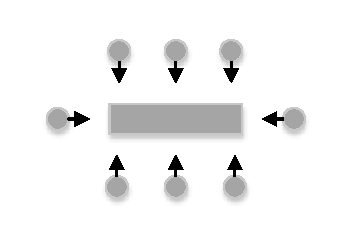
\includegraphics[width=0.5\textwidth]{MoveToTargetTraining.pdf}
\caption{Visualization of the eight training positions for the \textit{Move to Target} task. The circles indicate the relative starting positions of the actuator, while the arrows indicate the used action primitive.}
\label{fig:moveToTargetTraining}
\end{figure}

The training runs are performed by placing the actuator in a suitable starting position before applying a constant action primitive directed towards the block.
The used action primitives all have a norm of $0.5\frac{m}{s}$.

After training, both the actuator and the block are returned to their initial position. The block is located \m{0.25} above the global origin without any rotation, while the actuator is placed directly on top of the global origin.
Figure \ref{fig:moveToTargetScenario} visualizes the situation where the actuator just starts moving after training. The transparent light blue block symbolizes the target configuration of the block.

\begin{figure}
\centering
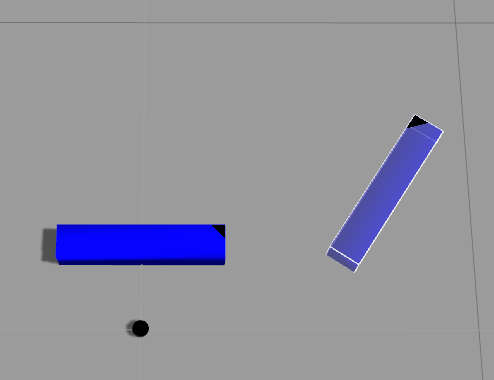
\includegraphics[width=0.5\textwidth]{MoveToTargetScenario.png}
\caption{Visualization of the \textit{Move to Target} task after training. The transparent light blue block indicates the desired target configuration. The blocks have been marked with the black corner to distinguish their orientation.}
\label{fig:moveToTargetScenario}
\end{figure}

\subsection{Evaluation criteria}

The performance of the inverse model is measured by the number of actions required to reach the target. If the target has not been reached within the allowed number of steps, the remaining difference is recorded. Similar to the previous task, position and orientation differences are recorded separately.

%TODO still want to do that?
%Furthermore, the average change in position and orientation per performed action is reported in order to judge the quality of the selected action primitives.

The models are tested with four targets which are shown in figure  \ref{fig:targetPositions}. All target configurations have the same positional difference to the starting position (\m{0.6} in either x direction and \m{0.7} in either y direction) but different orientations: 
\begin{itemize}
\item Target 1: \rad{-2.1}
\item Target 2: \rad{0.75}
\item Target 3: \rad{0.0} 
\item Target 4: \rad{3.1415}
\end{itemize}
For each target, the model is trained separately on the same training set in order to ensure comparability between the targets.

The testing of each target configuration is repeated 5 times and the averages over these runs are reported where possible.

\begin{figure}
\centering
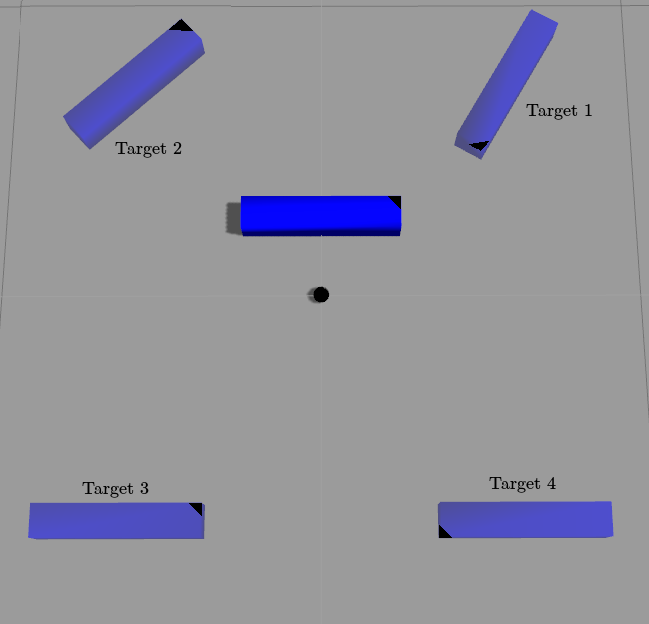
\includegraphics[width=0.5\textwidth]{MoveToTargetTargets.png}
\caption{Visualization of the four target configurations for the \textit{Move to Target} task. The black corners indicate the block's rotation.}
\label{fig:targetPositions}
\end{figure}

\subsection{Results}

The results for the interaction models are presented in table \ref{tab:moveToTargetInteractionResults} while the results for the object state with gating function model are presented in table \ref{tab:moveToTargetGateResults}.

\begin{table} %USE V2 sigma 0.05
	\centering
	\begin{tabular*}{\textwidth}{@{\extracolsep{\fill}} c c c c c } %c c}
			\hline \textbf{Target} & \textbf{Reached} & \textbf{Pos} & \textbf{Ori} & \textbf{\# steps} \\%& \textbf{Avg pos} & \textbf{Avg ori} \\ 
			\hline \hline 
			 Target 1 & 3 & 0.55 & 0.002 & 2689.2 (2482) \\ %&  & \\
			 Target 2 & 4 & 0.01 & 0.023 & 2430.4 (2288) \\ %& &  \\  
			 Target 3 & 5 & - & - & 1377.6 \\ %& &  \\  
			 Target 4 & 2 & 0.55 & 2.04 & 2492.2 (1730.5) \\ %& &  \\  
			\hline 
	\end{tabular*} 
	\caption{Evaluation results for the \textit{Move to Target} task for the interaction model. Pos and Ori columns represent the remaining error in position [m] and orientation [rad] respectively for the runs that did not reach the target. The number of steps in brackets represents the average over the runs that reached the target.}
	\label{tab:moveToTargetInteractionResults}
\end{table}

The object state with gating function reaches the targets in most cases within the allowed number of steps. Only target one was not reached in one run, however the remaining distance was quite small.

\begin{table}
	\centering
	\begin{tabular*}{\textwidth}{@{\extracolsep{\fill}} c c c c c } %c c}
			\hline \textbf{Target} & \textbf{Reached} & \textbf{Pos} & \textbf{Ori} & \textbf{\# steps} \\ %&  \textbf{Avg pos} & \textbf{Avg ori} \\ 
			\hline \hline 
			 Target 1 & 4 & 0.01 & 0.002 & 2271 (2088.8) \\ %& & \\
			 Target 2 & 5 & - & - & 1695 \\ %& &  \\  
			 Target 3 & 5 & - & - & 1147.4 \\ %& &  \\  
			 Target 4 & 5 & - & - & 1597.4 \\ %& &  \\  
			\hline 
	\end{tabular*} 
	\caption{Evaluation results for the \textit{Move to Target} task for the gate model. Pos and Ori columns represent the remaining error in position [m] and orientation [rad] respectively for the runs that did not reach the target. The number of steps in brackets represents the average over the runs that reached the target.}
	\label{tab:moveToTargetGateResults}
\end{table}

No target is never reached, but the interaction model had a few problems reaching the first and fourth targets. Looking at the combined error of position and orientation for the runs that did not reach the first and fourth target in detail revealed that in both cases, the model was not able to push the object straight without changing its orientation. The 2 runs that did not reach Target 1 as well as an exemplary third run that did reach can be seen in figure \ref{fig:moveToTargetInteractionT1Detail}.
In both failed runs, the model first reduces the difference in orientation successfully. However afterwards, it only manages to reduce the positional difference rotating the object away from the target orientation.

Snapshots of a successful run towards Target 1 performed by the object state model can be seen in figure \ref{fig:moveToTargetRun}. The image shows how the model first turns the object in the correct orientation. Afterwards the model pushes the object upwards and then towards the right. Finally some minor adjustments regarding the orientation and the position are made.

\begin{figure}
\centering
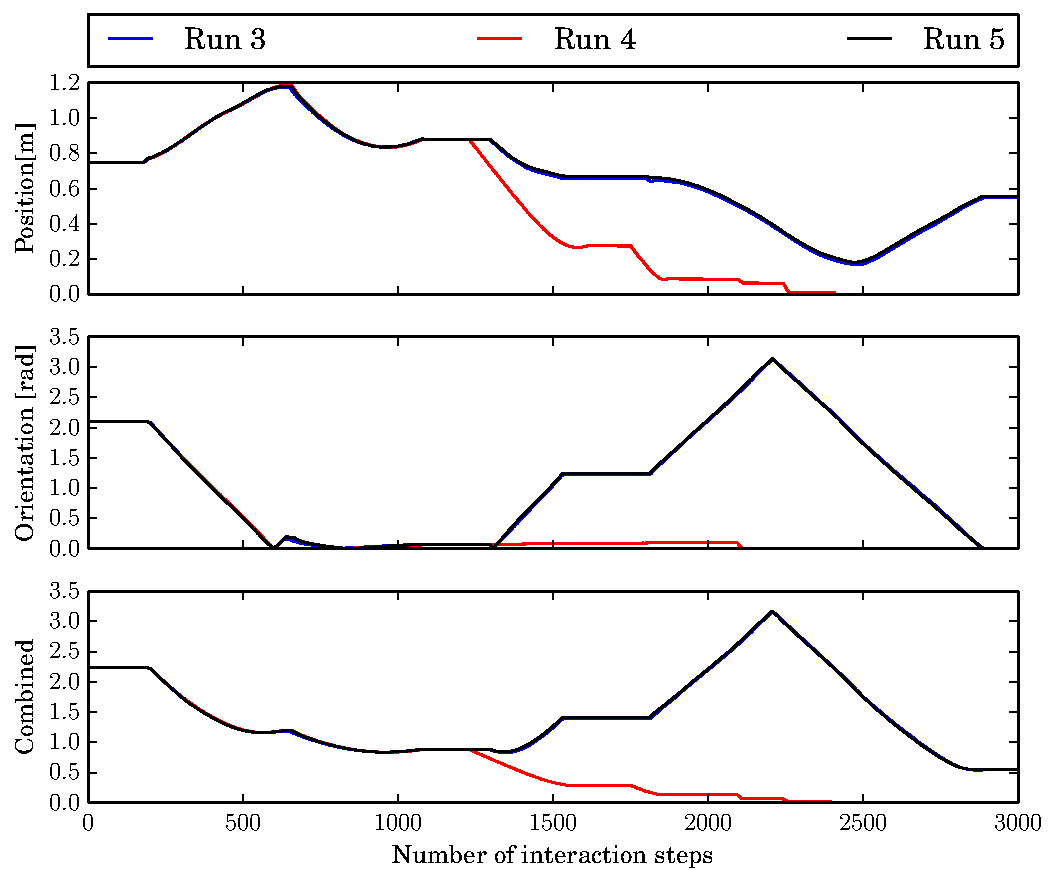
\includegraphics[width=0.8\textwidth]{MoveToTargetInteractionT1Detail.pdf}
\caption{Detailed view of three runs towards Target 1 performed by the interaction state model. The two runs that did not reach the target as well as one successful one are presented. The errors in position and orientation as well as the combined error over the interaction steps are shown.}
\label{fig:moveToTargetInteractionT1Detail}
\end{figure}

\begin{figure}
\centering
\includegraphics[width=\textwidth]{MoveToTargetRun.png}
\caption{Several snapshots from a run towards Target 1 by the object state model.
The run started at the image at the top left and finished at the bottom right.
There are around 50-150 updates in between two frames. The transparent block represents the target configuration.}
\label{fig:moveToTargetRun}
\end{figure}


%Two runs, including the one that did not quite reach the target for the object state model are visualized in figure \ref{fig:moveToTargetGateT1Detail}.
%
%\begin{figure}
%\centering
%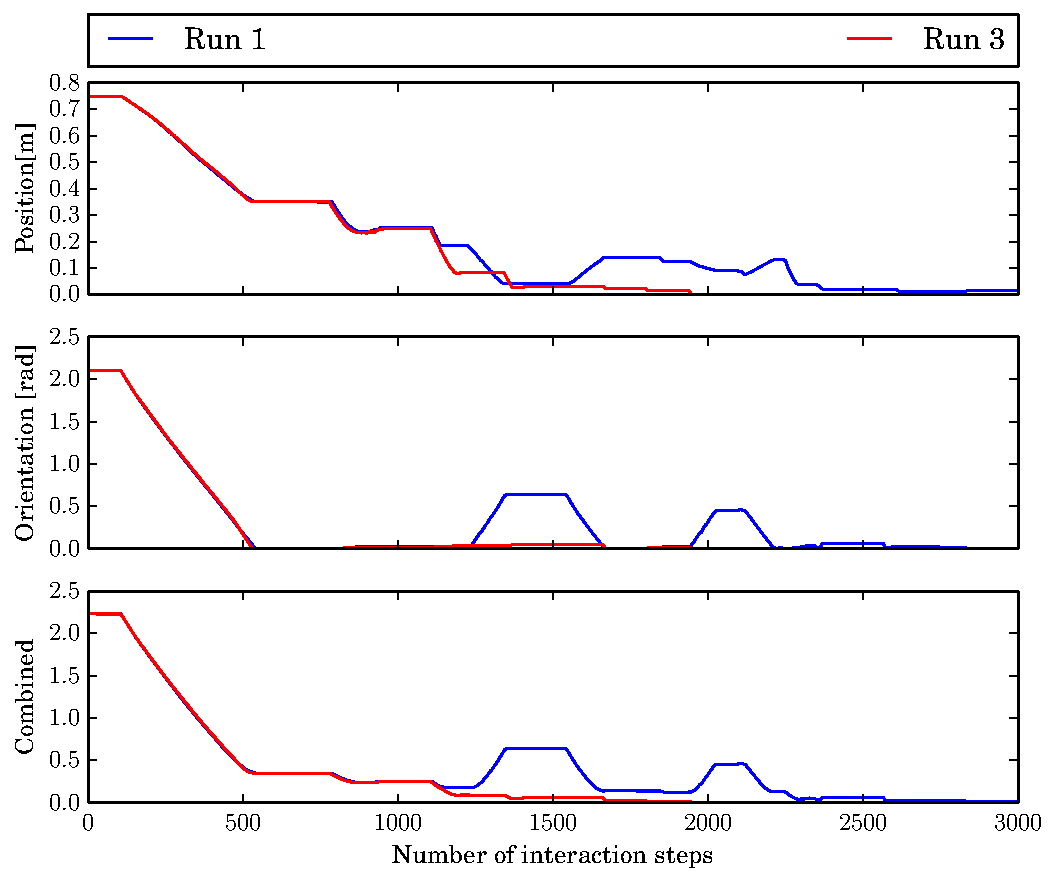
\includegraphics[width=0.8\textwidth]{MoveToTargetGateT1Detail.pdf}
%\caption{Detailed view of two runs towards Target 1 performed by the object state model. The errors in position and orientation as well as the combined error over the interaction steps are shown.}
%\label{fig:moveToTargetGateT1Detail}
%\end{figure}
%
%The plateaus that can be seen in the blue run indicate circling movements






